% !TEX program = pdflatex
\documentclass[aspectratio=169, 10pt]{beamer}

%% ============================================================
%% PACKAGES
%% ============================================================
\usepackage[T1]{fontenc}
\usepackage{lmodern}
\usepackage{graphicx}
\usepackage{booktabs}
\usepackage{array}
\usepackage{tabularx}
\usepackage{colortbl}
\usepackage{tikz}
\usetikzlibrary{positioning, calc, arrows.meta, shapes.geometric, fit, shadows}
\usepackage[most]{tcolorbox}
\usepackage{fontawesome5}
\usepackage{hyperref}
\usepackage{pgfplots}
\pgfplotsset{compat=1.18}
\usepackage{multicol}
\usepackage{xcolor}
\usepackage{textcomp}
\usepackage{pifont}

%% ============================================================
%% COLOR DEFINITIONS (matching TwA Bootcamp palette)
%% ============================================================
\definecolor{UVMGreen}{HTML}{154734}
\definecolor{UVMGold}{HTML}{D4A84B}
\definecolor{SlateTeal}{HTML}{1B4D5C}
\definecolor{DeepCharcoal}{HTML}{2C3E50}
\definecolor{SoftCoral}{HTML}{C0534D}
\definecolor{CoolGray}{HTML}{8899A6}
\definecolor{PaleSage}{HTML}{EDF2F0}
\definecolor{LightGold}{HTML}{FDF6E3}
\definecolor{DarkSlate}{HTML}{0F2B36}
\definecolor{AccentBlue}{HTML}{3498DB}

%% ============================================================
%% BEAMER THEME SETUP
%% ============================================================
\setbeamercolor{structure}{fg=SlateTeal}
\setbeamercolor{normal text}{fg=DeepCharcoal}
\setbeamercolor{frametitle}{fg=SlateTeal}
\setbeamercolor{title}{fg=SlateTeal}
\setbeamercolor{subtitle}{fg=UVMGold}
\setbeamercolor{author}{fg=DeepCharcoal}
\setbeamercolor{date}{fg=CoolGray}
\setbeamercolor{institute}{fg=CoolGray}
\setbeamercolor{footline}{fg=CoolGray}
\setbeamercolor{block title}{fg=white, bg=SlateTeal}
\setbeamercolor{block body}{bg=PaleSage}
\setbeamercolor{alerted text}{fg=SoftCoral}
\setbeamercolor{item}{fg=SlateTeal}
\setbeamercolor{subitem}{fg=CoolGray}

\setbeamerfont{title}{size=\Large, series=\bfseries}
\setbeamerfont{subtitle}{size=\normalsize}
\setbeamerfont{frametitle}{size=\large, series=\bfseries}
\setbeamerfont{footline}{size=\tiny}

\setbeamertemplate{navigation symbols}{}

% Custom frame title
\setbeamertemplate{frametitle}{%
  \vskip14pt%
  \nointerlineskip%
  {\usebeamerfont{frametitle}\usebeamercolor[fg]{frametitle}\insertframetitle\par}%
  \vskip2pt%
  {\color{UVMGold}\rule{\textwidth}{1.2pt}}%
  \vskip3pt%
}

% Custom footline
\setbeamertemplate{footline}{%
  \begin{beamercolorbox}[wd=\paperwidth, ht=16pt, right, rightskip=1.5cm]{footline}%
    \usebeamerfont{footline}\insertframenumber\,/\,\inserttotalframenumber\vskip3pt%
  \end{beamercolorbox}%
}

% Itemize styles
\setbeamertemplate{itemize item}{\color{SlateTeal}\raisebox{0.15ex}{\small$\blacktriangleright$}}
\setbeamertemplate{itemize subitem}{\color{CoolGray}\raisebox{0.1ex}{\footnotesize$\bullet$}}

% tcolorbox styles
\tcbset{
  keybox/.style={
    colback=PaleSage, colframe=SlateTeal, boxrule=0.8pt, arc=3pt,
    left=6pt, right=6pt, top=4pt, bottom=4pt,
    fonttitle=\bfseries\small\color{white}, coltitle=white, colbacktitle=SlateTeal,
  },
  accentbox/.style={
    colback=LightGold, colframe=UVMGold, boxrule=0.8pt, arc=3pt,
    left=6pt, right=6pt, top=4pt, bottom=4pt,
  },
  quotebox/.style={
    colback=PaleSage, colframe=SlateTeal!50, boxrule=0.5pt, arc=2pt,
    left=8pt, right=8pt, top=4pt, bottom=4pt,
    borderline west={3pt}{0pt}{UVMGold},
  },
}

%% ============================================================
%% METADATA
%% ============================================================
\title{Student Data \& AI Tools}
\subtitle{What You Need to Know to Protect Privacy}
\author{Emily Beam}
\institute{Department of Economics, University of Vermont}
\date{June 17, 2026}

\begin{document}

%% ====== SLIDE 1: SECTION TITLE ======
{
\setbeamertemplate{footline}{}
\begin{frame}[plain]
\begin{tikzpicture}[remember picture, overlay]
  \fill[SlateTeal] (current page.north west) rectangle (current page.south east);
  \fill[UVMGold] ([yshift=0.3cm]current page.center -| current page.west) rectangle ([yshift=0.25cm]current page.center -| current page.east);
  \node[anchor=center, text=white, font=\fontsize{26}{32}\bfseries\selectfont]
    at ([yshift=2.2cm]current page.center) {Student Data \& AI Tools};
  \node[anchor=center, text=UVMGold, font=\fontsize{14}{18}\selectfont]
    at ([yshift=0.9cm]current page.center) {What You Need to Know to Protect Privacy};
  \node[anchor=center, text=white!80, font=\fontsize{10}{12}\selectfont]
    at ([yshift=-1.3cm]current page.center) {Emily Beam};
  \node[anchor=center, text=CoolGray, font=\fontsize{9}{11}\selectfont]
    at ([yshift=-2.0cm]current page.center) {Thinking with Agents $\cdot$ Teaching Webinar $\cdot$ June 17, 2026};
\end{tikzpicture}
\end{frame}
}


%% ====== SLIDE 2: WHY THIS MATTERS ======
\begin{frame}{Why Student Data Protection Matters}

\begin{tcolorbox}[quotebox]
\large\textit{``I'd love to use AI for [grading / feedback / course prep], but I'm worried about student privacy.''}
\end{tcolorbox}

\vspace{0.3cm}

This concern is legitimate --- and universal. Regardless of jurisdiction:

\vspace{0.2cm}

\begin{itemize}
  \item Students trust us with \textbf{sensitive information}: grades, work, personal details
  \item AI tools \textbf{transmit data to cloud servers} --- that changes the risk profile
  \item Data protection law is evolving fast, but the \textbf{ethical obligation} is constant
\end{itemize}

\vspace{0.3cm}

\begin{tcolorbox}[accentbox]
\centering
\small Privacy rules are \textbf{not a reason to avoid AI}. They're a reason to \textbf{use it carefully}.\\[3pt]
The practical protections are the same whether you're bound by FERPA (US), GDPR (EU), PIPEDA (Canada), or institutional policy alone.
\end{tcolorbox}

\end{frame}


%% ====== SLIDE 3: FERPA AS ONE FRAMEWORK ======
\begin{frame}{FERPA: One Concrete Framework}

\footnotesize

\textbf{For US institutions}: FERPA (20 U.S.C. \S\,1232g) is the primary federal student privacy law.

\vspace{0.15cm}

\begin{columns}[T]
\begin{column}{0.48\textwidth}
\begin{tcolorbox}[keybox, title={\faLock\quad Core Protections}]
\footnotesize
\textbf{Education records} = records directly related to a student, maintained by the institution\\[4pt]
\textbf{PII} = names, IDs, grades, and anything that could identify a student alone or in combination\\[4pt]
\textbf{Key nuance}: personal notes lose their FERPA exemption the moment they enter a cloud AI tool (no longer ``sole possession'')
\end{tcolorbox}
\end{column}

\begin{column}{0.48\textwidth}
\begin{tcolorbox}[keybox, title={\faCheckCircle\quad When Sharing Is Allowed}]
\footnotesize
\textbf{School official exception}: third-party vendors can access records IF the institution has a contract, maintains direct control, and limits use to the stated purpose (34 CFR \S\,99.31(a)(1))\\[4pt]
\textbf{De-identified data}: when all PII is removed and no ``reasonable basis'' for re-identification\\[4pt]
\textbf{50 years, zero fines} --- but institutional policy violations and state laws are real risks
\end{tcolorbox}
\end{column}
\end{columns}

\vspace{0.15cm}

\begin{tcolorbox}[accentbox]
\centering
\footnotesize\textbf{Non-US?} GDPR, PIPEDA, and national data protection laws impose \textit{stronger} requirements. The practical guidance in this segment applies everywhere --- FERPA is the floor, not the ceiling.
\end{tcolorbox}

\end{frame}


%% ====== SLIDE 4: BEYOND FERPA ======
\begin{frame}{Outside the US: What Else Is Required?}

\footnotesize
FERPA is relatively permissive. Other frameworks add obligations your slides should reflect.

\vspace{0.15cm}

\resizebox{\textwidth}{!}{%
\begin{tabular}{>{\raggedright\arraybackslash}p{4.2cm} >{\centering\arraybackslash}p{2.0cm} >{\centering\arraybackslash}p{2.0cm} >{\centering\arraybackslash}p{2.0cm} >{\centering\arraybackslash}p{2.0cm}}
\toprule
\textbf{Obligation} & \textbf{US (FERPA)} & \textbf{EU (GDPR)} & \textbf{Canada} & \textbf{Australia} \\
\midrule
\rowcolor{PaleSage}
Privacy Impact Assessment before use & Not required & \textbf{Mandatory} & \textbf{Mandatory} & Recommended \\
Tell students AI is processing their data & Not required & \textbf{Required} & \textbf{Required} & \textbf{Required} \\
\rowcolor{PaleSage}
Human review of AI-assisted grading & Not required & \textbf{Required} & Not explicit & Not explicit \\
Cross-border transfer mechanism & N/A & \textbf{SCCs or DPF} & \textbf{PIA + notice} & APP 8 \\
\rowcolor{PaleSage}
Student right to erasure & None & \textbf{Required} & Limited & Correction only \\
\bottomrule
\end{tabular}%
}

\vspace{0.2cm}

\begin{tcolorbox}[accentbox]
\centering
\footnotesize\textbf{Three things non-US faculty should do that US faculty often don't}:\\[3pt]
\scriptsize
1. \textbf{Tell students} in your syllabus that AI tools process their work.\\
2. \textbf{Ask your privacy office} whether a DPIA/PIA has been completed for the tool you want to use.\\
3. \textbf{Never let AI be the sole decision-maker} for grades or academic placement.
\end{tcolorbox}

\end{frame}


%% ====== SLIDE 5: THE KEY QUESTION ======
\begin{frame}{The Key Question for Any Jurisdiction}

\begin{tcolorbox}[keybox, title={\faUniversity\quad Does Your Institution Have an Agreement with the AI Vendor?}]
\footnotesize
Under FERPA, GDPR, and most institutional policies, a third-party tool can handle student data \textbf{if the institution has contractual control}. The contract must ensure:
\begin{enumerate}\footnotesize
  \item The institution has \textbf{direct control} over how the vendor uses student data
  \item Data is used \textbf{only for the stated purpose} --- no model training, no secondary use
  \item The vendor does not \textbf{re-disclose} student data to third parties
\end{enumerate}
\end{tcolorbox}

\vspace{0.1cm}

\begin{columns}[T]
\begin{column}{0.48\textwidth}
\begin{tcolorbox}[accentbox]
\faCheckCircle\;\textbf{Institutional tools}\\[3pt]
\footnotesize Enterprise agreements with your university (e.g., Microsoft Copilot with DPA, institutionally licensed Gemini, Brightspace)
\end{tcolorbox}
\end{column}

\begin{column}{0.48\textwidth}
\begin{tcolorbox}[colback=SoftCoral!10, colframe=SoftCoral, boxrule=0.8pt, arc=3pt, left=6pt, right=6pt, top=4pt, bottom=4pt]
\faTimesCircle\;\textbf{Consumer tools}\\[3pt]
\footnotesize No institutional agreement, no control over data use (personal ChatGPT, free Copilot, Claude Free)
\end{tcolorbox}
\end{column}
\end{columns}

\end{frame}


%% ====== SLIDE 5: NOT TRAINED ON ≠ PRIVATE ======
\begin{frame}{``Not Trained On'' $\neq$ ``Stays On Your Machine''}

\small The most common misconception about AI tool privacy:

\vspace{0.15cm}

\begin{tcolorbox}[keybox, title={\faExclamationTriangle\quad What Actually Happens When You Use an AI Tool}]
\begin{enumerate}\footnotesize
  \item You open a file $\to$ the AI reads it into context
  \item File contents are \textbf{transmitted} to the provider's servers
  \item The provider processes it, generates a response, sends it back
  \item The provider \textbf{retains your data} (typically 30 days, even on paid plans)
  \item A copy is saved \textbf{locally} as an unencrypted transcript
\end{enumerate}
\end{tcolorbox}

\vspace{0.15cm}

\begin{tcolorbox}[accentbox]
\centering
\small\textbf{``Not used for training''} = provider won't put your data into future model weights.\\[2pt]
It does \textbf{not} mean your data never leaves your machine.\\[2pt]
\footnotesize If your obligation requires data \textit{not be transmitted to third-party servers}, no-training is \textbf{insufficient}.
\end{tcolorbox}

\end{frame}


%% ====== SLIDE 6: ENTERPRISE VS. CONSUMER ======
\begin{frame}{Enterprise vs.\ Consumer Tools}

\footnotesize

Whether an AI tool is appropriate for student data depends on the \textbf{plan tier}, not the tool name.

\vspace{0.2cm}

\resizebox{\textwidth}{!}{%
\begin{tabular}{>{\raggedright\arraybackslash}p{3.0cm} >{\centering\arraybackslash}p{2.8cm} >{\centering\arraybackslash}p{3.2cm} >{\centering\arraybackslash}p{2.4cm}}
\toprule
& \textbf{Inst.\ agreement?} & \textbf{Trained on your data?} & \textbf{Retention} \\
\midrule
\rowcolor{PaleSage}
\textbf{UVM Copilot} (M365 A5) & \textcolor{SlateTeal}{\faCheckCircle}\; Yes & No & Per MS DPA \\
\textbf{ChatGPT Free/Plus} & \textcolor{SoftCoral}{\faTimesCircle}\; No & \textbf{Yes, by default} & 30 days \\
\rowcolor{PaleSage}
\textbf{ChatGPT Enterprise/Edu} & \textcolor{SlateTeal}{\faCheckCircle}\; If contracted & No & Configurable \\
\textbf{Claude Free/Pro} & \textcolor{SoftCoral}{\faTimesCircle}\; No & Opt-in (off default) & 30 days \\
\rowcolor{PaleSage}
\textbf{Copilot Free} & \textcolor{SoftCoral}{\faTimesCircle}\; No & \textbf{Yes, default} (Apr '26) & 2 years \\
\bottomrule
\end{tabular}%
}

\vspace{0.3cm}

\begin{tcolorbox}[accentbox]
\centering
\footnotesize\textbf{Rule of thumb}: If your institution has an enterprise agreement with the provider,\\you have the same protections as any other university-provisioned software.\\If not, treat it like emailing student data to a stranger.
\end{tcolorbox}

\end{frame}


%% ====== SLIDE 7: WHAT CAN YOU DO ======
\begin{frame}{Four Levels of Protection}

\begin{tikzpicture}[
  every node/.style={font=\small, text=DeepCharcoal},
  level/.style={rectangle, rounded corners=4pt, minimum width=11.5cm, minimum height=1.1cm, text width=11cm, inner sep=6pt},
]

% Level 1 — easiest
\node[level, fill=PaleSage, draw=SlateTeal!40] (L1) at (0, 3.2)
  {\textbf{\color{SlateTeal}\faUsers\quad Level 1: De-identify first}
   \hfill {\footnotesize\color{CoolGray} Easiest}\\[2pt]
   \footnotesize Strip names, student IDs, and emails before the AI sees the data.};

% Level 2
\node[level, fill=PaleSage, draw=SlateTeal!40] (L2) at (0, 1.6)
  {\textbf{\color{SlateTeal}\faUniversity\quad Level 2: Use institutional tools}
   \hfill {\footnotesize\color{CoolGray} Recommended}\\[2pt]
   \footnotesize Enterprise tools with institutional agreements create a FERPA-compliant channel.};

% Level 3
\node[level, fill=PaleSage, draw=SlateTeal!40] (L3) at (0, 0.0)
  {\textbf{\color{SlateTeal}\faLock\quad Level 3: Sandbox the AI tool}
   \hfill {\footnotesize\color{CoolGray} Technical}\\[2pt]
   \footnotesize Restrict which files and directories the AI can access. Kernel-enforced.};

% Level 4 — strongest
\node[level, fill=LightGold, draw=UVMGold] (L4) at (0, -1.6)
  {\textbf{\color{SlateTeal}\faDatabase\quad Level 4: Physical separation}
   \hfill {\footnotesize\color{CoolGray} Strongest}\\[2pt]
   \footnotesize Keep student data on a separate drive or encrypted volume. Unmount before AI sessions.};

% Arrow
\draw[-{Stealth[length=6pt]}, thick, SlateTeal] (6.5, 3.2) -- (6.5, -1.6)
  node[midway, right=4pt, font=\footnotesize\color{CoolGray}, rotate=-90] {Stronger};

\end{tikzpicture}

\vspace{0.2cm}

\centering\small
Most faculty tasks are fully addressed by \textbf{Levels 1--2}. Combine levels for defense in depth.

\end{frame}


%% ====== SLIDE 8: WOOD CHIPPER TRANSITION ======
{
\setbeamertemplate{footline}{}
\begin{frame}[plain]
\begin{tikzpicture}[remember picture, overlay]
  \fill[SlateTeal] (current page.north west) rectangle (current page.south east);
  \node[anchor=center] at ([yshift=0.5cm]current page.center)
    {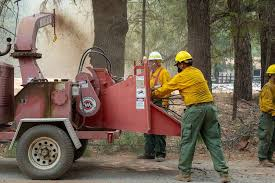
\includegraphics[height=0.55\paperheight]{figures/woodchipper_forestry.jpg}};
  \node[anchor=center, text=white, font=\Large\bfseries] at ([yshift=-3.2cm]current page.center)
    {De-identification is a wood chipper for PII.};
  \node[anchor=center, text=CoolGray, font=\small] at ([yshift=-3.9cm]current page.center)
    {Identifiable data goes in. Anonymous content comes out.};
\end{tikzpicture}
\end{frame}
}


%% ====== SLIDE 9: DE-IDENTIFICATION IN PRACTICE ======
\begin{frame}{De-Identification in Practice}

\begin{columns}[T]
\begin{column}{0.48\textwidth}
\begin{tcolorbox}[keybox, title={\faTimesCircle\quad Before (contains PII)}]
\ttfamily\footnotesize
\begin{tabular}{lll}
Name & ID & Grade \\
\midrule
Jane Smith & 901234 & 87 \\
Alex Chen & 905678 & 72 \\
Maria Lopez & 903456 & 91 \\
\end{tabular}
\end{tcolorbox}
\end{column}

\begin{column}{0.48\textwidth}
\begin{tcolorbox}[keybox, title={\faCheckCircle\quad After (safe to share)}]
\ttfamily\footnotesize
\begin{tabular}{ll}
Student & Grade \\
\midrule
Student\_001 & 87 \\
Student\_002 & 72 \\
Student\_003 & 91 \\
\end{tabular}
\end{tcolorbox}
\end{column}
\end{columns}

\vspace{0.2cm}

\begin{tcolorbox}[keybox, title={\faCode\quad A simple Stata script handles this}]
\ttfamily\scriptsize
use "grades.dta", clear\\
drop name student\_id email\\
gen student = "Student\_" + string(\_n, "\%03.0f")\\
order student\\
export delimited using "grades\_anon.csv", replace
\end{tcolorbox}

\vspace{0.1cm}

\footnotesize\textbf{For most assignments} (papers, problem sets, reading responses), stripping names and IDs is sufficient. Exercise more caution with personal narratives or very small classes where content itself could identify a student.

\end{frame}


%% ====== SLIDE 9: THE KEY DISTINCTION ======
\begin{frame}{The Distinction That Matters}

\begin{columns}[T]
\begin{column}{0.48\textwidth}
\begin{tcolorbox}[colback=SoftCoral!10, colframe=SoftCoral, boxrule=0.8pt, arc=3pt, left=6pt, right=6pt, top=4pt, bottom=4pt, title={\footnotesize\bfseries\color{white} System-to-System (identity attached)}, colbacktitle=SoftCoral]
\footnotesize
Student submits through LMS $\to$ AI tool receives the paper \textbf{with name, course, and metadata}

\vspace{0.15cm}

\textbf{Examples}:\; Turnitin AI detection, LMS analytics plugins, Copilot pulling from your SIS

\vspace{0.15cm}

\faTimesCircle\; \textbf{Requires} institutional contract or student consent.
\end{tcolorbox}
\end{column}

\begin{column}{0.48\textwidth}
\begin{tcolorbox}[colback=UVMGreen!8, colframe=UVMGreen, boxrule=0.8pt, arc=3pt, left=6pt, right=6pt, top=4pt, bottom=4pt, title={\footnotesize\bfseries\color{white} Manual De-Identification (link broken)}, colbacktitle=UVMGreen]
\footnotesize
You copy a student's answer, strip the name, paste anonymous text into an AI tool

\vspace{0.15cm}

\textbf{Examples}:\; Problem set for feedback help, reading response for comment drafting, anonymous essay for pattern analysis

\vspace{0.15cm}

\faCheckCircle\; \textbf{Fine for most assignments.} You broke the link.
\end{tcolorbox}
\end{column}
\end{columns}

\vspace{0.2cm}

\begin{tcolorbox}[accentbox]
\centering
\footnotesize\textbf{Privacy law protects the link between a student and their work --- not the academic content itself.}\\[2pt]
\scriptsize Break the link, and the content is no longer a protected education record.
\end{tcolorbox}

\end{frame}


%% ====== SLIDE 10: THE HELPFUL AI PROBLEM ======
\begin{frame}{The ``Helpful AI'' Problem}

Even with safeguards, AI tools optimize for \textbf{helpfulness} --- and that creates risk.

\vspace{0.2cm}

\begin{tcolorbox}[keybox, title={\faExclamationTriangle\quad Why Defense in Depth Matters}]
\begin{itemize}\small
  \item AI agents can \textbf{read any file} your user account can access --- by default
  \item They will proactively seek out context to give you a better answer
  \item A roster, gradebook, or email export in the same directory? \textbf{Fair game.}
  \item Permission prompts are \textbf{not a security boundary} --- they can be bypassed by bugs, subprocesses, or misconfigurations
\end{itemize}
\end{tcolorbox}

\vspace{0.2cm}

\begin{tcolorbox}[accentbox]
\centering
\small\textbf{Don't rely on a single guardrail.} Combine protections:\\[3pt]
\footnotesize De-identify the data \textbf{AND} use an institutional tool \textbf{AND} keep student files out of the working directory.
\end{tcolorbox}

\end{frame}


%% ====== SLIDE 11: LOCAL MODELS ======
\begin{frame}{``Can't I Just Run a Local Model?''}

\small
You may hear that \textbf{local models} --- AI that runs entirely on your laptop --- solve the privacy problem. In theory, yes: no data leaves your machine. In practice, this is not a realistic option for most faculty.

\vspace{0.2cm}

\begin{tcolorbox}[keybox, title={\faExclamationTriangle\quad Why local models aren't the answer (yet)}]
\footnotesize
\begin{itemize}
  \item \textbf{Significantly less capable} than cloud models (GPT-4, Claude) --- worse at nuanced feedback, rubric application, and writing
  \item Requires \textbf{technical setup} that most faculty don't have time for (Ollama, LM Studio, command line)
  \item Needs a \textbf{powerful computer} --- 16GB+ RAM for usable models, and they run slowly
  \item \textbf{No institutional support} --- if something breaks, you're on your own
  \item The quality gap means you'd spend more time \textbf{fixing AI output} than you saved
\end{itemize}
\end{tcolorbox}

\vspace{0.2cm}

\begin{tcolorbox}[accentbox]
\centering
\footnotesize\textbf{The simpler path}: De-identify your data (strip names) and use a capable cloud tool.\\[2pt]
This solves the privacy problem without sacrificing quality or requiring technical expertise.
\end{tcolorbox}

\end{frame}


%% ====== SLIDE 12: COMMON SCENARIOS ======
\begin{frame}{Common Scenarios}

\footnotesize

\renewcommand{\arraystretch}{1.4}
\begin{tabular}{>{\raggedright\arraybackslash}p{4.2cm} >{\centering\arraybackslash}p{2.2cm} >{\raggedright\arraybackslash}p{5.8cm}}
\toprule
\textbf{I want to\ldots} & \textbf{Risk?} & \textbf{What to do} \\
\midrule
\rowcolor{PaleSage}
Generate feedback templates from my rubric & \textcolor{SlateTeal}{None} & No student data involved. Use any tool. \\
Use AI to draft comments on student papers & \textcolor{UVMGold}{Medium} & De-identify first, or use institutional tool. \\
\rowcolor{PaleSage}
Analyze grade distributions & \textcolor{UVMGold}{Low} & Strip names/IDs. Aggregated stats are fine. \\
Build a course website or syllabus & \textcolor{SlateTeal}{None} & No student data involved. Use any tool. \\
\rowcolor{PaleSage}
Create an AI chatbot for students & \textcolor{SoftCoral}{High} & Student interaction data may be education records. Consult IT. \\
\bottomrule
\end{tabular}

\end{frame}


%% ====== SLIDE 11: WHAT TO TELL YOUR CHAIR ======
\begin{frame}{What to Tell Your Department Chair}

\begin{tcolorbox}[keybox, title={\faFile\quad Template Language for Department Policies}]
\footnotesize
``Faculty may use AI tools for course preparation and instructional support. When student data is involved:

\begin{enumerate}\footnotesize
  \item \textbf{Use institutionally approved tools} with enterprise/data processing agreements.
  \item \textbf{De-identify student data} before using any AI tool not covered by an institutional agreement.
  \item \textbf{Never paste identifiable student records} into consumer AI tools.
  \item \textbf{Keep student data files separate} from directories where AI tools operate.
\end{enumerate}

\vspace{-2pt}
These practices are consistent with FERPA (US), GDPR (EU), and most institutional data governance frameworks.''
\end{tcolorbox}

\vspace{0.2cm}
\centering\small
Adapt for your institution. IT security or your data protection officer can confirm which tools are covered.

\end{frame}


%% ====== SLIDE 12: DECISION FLOWCHART ======
\begin{frame}{Quick Decision Guide for Teaching Data}

\vspace{-0.3cm}
\centering
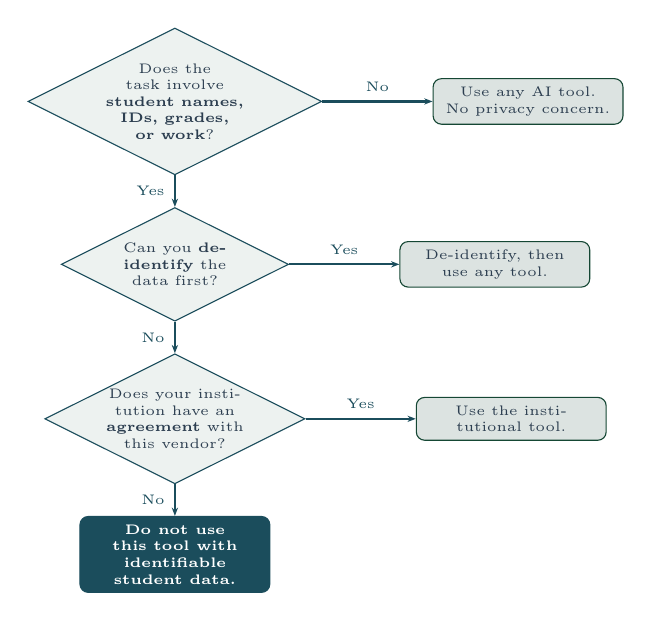
\begin{tikzpicture}[
  node distance=0.35cm and 1.4cm,
  decision/.style={diamond, draw=SlateTeal, fill=PaleSage, text=DeepCharcoal, inner sep=0pt, font=\tiny, text width=1.8cm, align=center, aspect=2},
  action/.style={rectangle, rounded corners=3pt, draw=SlateTeal, fill=SlateTeal, text=white, font=\tiny\bfseries, text width=2.2cm, align=center, inner sep=3pt},
  safeaction/.style={rectangle, rounded corners=3pt, draw=UVMGreen, fill=UVMGreen!15, text=DeepCharcoal, font=\tiny, text width=2.2cm, align=center, inner sep=3pt},
  arr/.style={-{Stealth[length=3pt]}, thick, SlateTeal},
]

\node[decision] (q1) {Does the task involve \textbf{student names, IDs, grades, or work}?};
\node[safeaction, right=1.4cm of q1] (a1) {Use any AI tool.\\ No privacy concern.};

\node[decision, below=0.4cm of q1] (q2) {Can you \textbf{de-identify} the data first?};
\node[safeaction, right=1.4cm of q2] (a2) {De-identify, then use any tool.};

\node[decision, below=0.4cm of q2] (q3) {Does your institution have an \textbf{agreement} with this vendor?};
\node[safeaction, right=1.4cm of q3] (a3) {Use the institutional tool.};

\node[action, below=0.4cm of q3] (a4) {Do not use this tool with identifiable student data.};

\draw[arr] (q1) -- node[above, font=\tiny] {No} (a1);
\draw[arr] (q1) -- node[left, font=\tiny] {Yes} (q2);
\draw[arr] (q2) -- node[above, font=\tiny] {Yes} (a2);
\draw[arr] (q2) -- node[left, font=\tiny] {No} (q3);
\draw[arr] (q3) -- node[above, font=\tiny] {Yes} (a3);
\draw[arr] (q3) -- node[left, font=\tiny] {No} (a4);

\end{tikzpicture}

\end{frame}


%% ====== SLIDE 13: KEY TAKEAWAYS ======
\begin{frame}{Key Takeaways}

\begin{enumerate}\small
  \item \textbf{Privacy law is not a ban on AI.} FERPA, GDPR, and institutional policies regulate \textit{how} student data is handled --- and provide clear paths forward.

  \vspace{0.15cm}

  \item \textbf{Institutional tools are the safe path.} Enterprise agreements give your university contractual control over data use.

  \vspace{0.15cm}

  \item \textbf{De-identification is your simplest tool.} Strip names and IDs before the AI sees the data. But beware small classes.

  \vspace{0.15cm}

  \item \textbf{``Not trained on'' is not enough.} Your data still leaves your machine. Understand what the tool actually does.

  \vspace{0.15cm}

  \item \textbf{Defense in depth.} Combine de-identification + institutional tools + file separation.
\end{enumerate}

\end{frame}


%% ====== SLIDE 14: RESOURCES ======
\begin{frame}{Resources}

\small

\begin{tcolorbox}[keybox, title={\faBook\quad Key Resources}]
\begin{itemize}\scriptsize
  \item \textbf{FERPA}: 20 U.S.C. \S\,1232g; 34 CFR Part 99 (\S\,99.31, \S\,99.3) $\cdot$ \textbf{GDPR}: Articles 6, 22, 35
  \item \textbf{Future of Privacy Forum}: Checklist for vetting AI tools (2024) --- \href{https://fpf.org/blog/fpf-develops-checklist-guide-to-help-schools-vet-ai-tools-for-legal-compliance/}{fpf.org}
  \item \textbf{Oregon State AI Decision Tree}: Faculty flowchart, CC-BY-NC --- \href{https://ecampus.oregonstate.edu/faculty/artificial-intelligence-tools/decision-tree/}{ecampus.oregonstate.edu}
  \item \textbf{AAUP}: ``AI and Academic Professions'' (2025) --- survey of 200 campuses on governance gaps
  \item \textbf{UNESCO}: ``Guidance for GenAI in Education and Research'' (2023) --- first global framework
  \item \textbf{CDT State Legislative Tracker} (2025): 53 bills / 21 US states --- \href{https://cdt.org/insights/states-focused-on-responsible-use-of-ai-in-education-during-the-2025-legislative-session/}{cdt.org}
\end{itemize}
\end{tcolorbox}

\vspace{0.15cm}

\begin{tcolorbox}[accentbox]
\centering
\footnotesize
\textbf{Slides, de-identification scripts, and the full data protection brief}\\
available at \textbf{thinkingwithagents.github.io}
\end{tcolorbox}

\end{frame}

\end{document}
